% !TeX root = RJwrapper.tex
\title{Log Likelihood Ratios for Common Statistical Tests Using the likelihoodR Package}
\author{by Peter Cahusac}

\maketitle

\abstract{
The \textbf{likelihoodR} package has been developed to allow users to obtain statistics according to the likelihood approach to statistical inference. Commonly used tests are available in the package, such as: \emph{t} tests, ANOVA, correlation, regression and a range of categorical analyses. In addition, there is a sample size calculator for \emph{t} tests, based upon the concepts of strength of evidence, and the probabilities of misleading and weak evidence.
}

\section{Introduction}

Maximum likelihood estimation (MLE) is well-understood and widely used throughout statistics. In contrast, the use of the likelihood function as a basis for inference is much less understood and even confused with MLE. As Edwards wrote in his excellent book : "At one recent international conference at which I laboured for three-quarters of an hour to make clear the advantages of likelihood inference, the chairman thanked me for my lecture on the Method of Maximum Likelihood" \citep{Edwards:1992} p 101. In the Epilogue of this book on p 212, Edwards says that MLE is “a red herring”. To clarify: MLE is used to estimate a parameter value according to a supposed probability distribution, while likelihood inference is used to compare two hypotheses through the ratio of their values on a likelihood function.\\

All the main statistical approaches to scientific inference (frequentist, Bayesian and information criterion) are based upon calculated probabilities. The frequentist approach, for example, typically uses a sampling distribution centred on a null hypothesis and calculates the probability of obtaining the observed value or values more extreme from the null. The likelihood approach, also known as the evidential approach, differs in that it is simply based upon the evidence provided by the observed data (not including more extreme values) and represented by the likelihood function. The ratio of the heights under the likelihood function according to the hypothesis values tested provides the likelihood ratio. To create a linear scale of evidence, the natural logarithm of this is taken to give us the log likelihood ratio, also known as the support, a term that was first defined by Harold Jeffreys \citep{Jeffreys:1936}.\\

The likelihood approach is not subject to the same criticisms often leveled at the frequentist and Bayesian approaches \citep{GoodmanRoyall:1988,Edwards:1992,Royall:1997,Goodman:1999,Dixon:2003,Dienes:2008,WassersteinLazar:2016,Lakens:2021}. Likelihood ratios provide objective measures of evidence between competing hypotheses, unaffected by the intentions of the investigator. Log likelihood ratio (\emph{support}, see below) values are proportional to the quantity of data, representing the weight of evidence. This means that support values from independent studies can simply be added together, e.g. for meta-analysis. Unlike other approaches based on probabilities, likelihood ratios are unaffected by transformations of variables.\\

Despite the apparent advantages of the evidential approach there is a dearth of available resources in statistical computing. None of the major commercial packages (e.g. SPSS, SAS, Minitab) provide likelihood ratios or support values. This should not be confused with the wide availability of likelihood ratio tests (also known as G-tests), which ultimately provide \emph{p} values according to the frequentist approach. 
Because virtually no software is available for analysis, this impacts on the use of the evidential approach in scientific reporting. This also impacts on the teaching of the evidential approach, which then negatively feeds back to reduced scientific reporting. The \textbf{likelihoodR} package for R \citep{likelihoodR} is an attempt to address this situation and calculations are based upon the recent book \citep{Cahusac:2020}. R \citep{ihaka:1996} is a widely used statistical platform with a huge variety of packages.\\

\section{Support}
The package always reports the support (log likelihood ratio). This relative evidence scale ranges from -$\infty$ to +$\infty$, with zero representing no evidence either way. A working interpretation for this scale has been offered by \citep{GoodmanRoyall:1988}, see Table 1. No threshold need be applied, and \emph{S} values are given to just one decimal place, e.g. 2.3.\\

\begin{table}[ht]  
\begin{center}  
\begin{tabular}{|l|l|}  
\textbf{\emph{S}} & \textbf{Interpretation of H$_{1}$ vs H$_{2}$}\\  
\hline  
0 & No evidence either way\\  
1 & Weak evidence\\
2 & Moderate evidence\\
3 & Strong evidence\\  
4 & Extremely strong evidence\\
\end{tabular}  
\caption{ Interpretation for values of \emph{S}, the support, calculated as the natural logarithm of the
likelihood ratio. Negative values would represent support for hypothesis values H$_{2}$ vs H$_{1}$. Typically, it is sufficient to
give \emph{S} to one decimal place.}  
\label{tab:Table1}  
\end{center}  
\end{table}

The support (\emph{S}) values reported in the package are distinct from the surprise/surprisal S-values described by \citep{Palm:2012} based on Shannon information theory, and that by \citep{Greenland:2019} produced by simply taking the negative log base 2 of the \emph{p} value.\\

The likelihood intervals are reported wherever possible and these are given in terms of support rather than likelihood ratio. A typical likelihood interval (support interval) is the \emph{S}-2 interval, which numerically often closely corresponds to the frequentist 95\% confidence interval \citep{Cahusac:2020}. The \emph{S}-2 interval represents an interval based upon e$^{-2}$ = 0.135 = 1 / 7.40 likelihood ratio interval. All the values within the interval would have a likelihood ratio of no less than 1 / 7.40, or an \emph{S} = -2. The \emph{S}-3 interval would be e$^{-3}$ = 0.05 = 1 / 20.09, and so on. Analyses also report other relevant statistics, such as \emph{t}, F and $\chi^{2}$, as well as the corresponding frequentist \emph{p} value.
Where possible the likelihood function is given, decorated with hypothesis parameter values shown as coloured lines. 
Currently there are 14 different statistical tests implemented by the package, the summary for each are given in Table 2 (listed alphabetically).\\ 

\begin{table}[ht]  
\begin{center}  
\begin{tabular}{ll}  
\hline  
\textbf{Function} & \textbf{Description}\\
\hline  
\texttt{L\_1way\_ANOVA} &  Independent samples one-way ANOVA\\  
\texttt{L\_1way\_cat} & One-way categorical data analysis for binomial and multinomial\\
\texttt{L\_1way\_RM\_ANOVA} & One-way repeated measures ANOVA\\
\texttt{L\_2S\_ttest} &  Independent samples \emph{t} test\\  
\texttt{L\_2way\_cat} & Two-way categorical data analysis\\
\texttt{L\_2way\_Factorial\_ANOVA} & Two-way independent samples factorial ANOVA\\
\texttt{L\_corr} & Bivariate normal correlation\\
\texttt{L\_efficacy} & Efficacy analysis for binomial categorical data\\
\texttt{L\_logistic\_regress} & Multiple logistic regression\\
\texttt{L\_OR} & Odds ratio\\
\texttt{L\_regress} & Bivariate regression for linear, quadratic and cubic comparisons\\
\texttt{L\_RR} & Relative risk\\
\texttt{L\_ttest} & One sample and related samples \emph{t} test\\
\texttt{L\_t\_test\_sample\_size} & Sample size calculation using the evidential approach for \emph{t} tests\\
\hline  
\end{tabular}  
\caption{ A summary of the functions available in the \textbf{likelihoodR} package}  
\label{tab:Table2}  
\end{center}  
\end{table} 


\section{Continuous data}

A range of tests for differences of continuous variables is available. One function \texttt{L\_ttest} performs a one sample and related samples test. As well as specifying the null value, two alternative hypothesis values can be specified, one in terms of the measurements used and the other in terms of Cohen's d.\\\\
\texttt{L\_ttest(data1, data2, null=0, d=0.5, alt.2=NULL, L.int=2, verb=TRUE)}\\\\
Where the arguments are:\\
\begin{tabular}{ll}  
data1 & a (non-empty) numeric vector of data values\\  
data2 & a (non-empty) numeric vector of data values for related sample, default = NULL\\  
null 	& value for the null hypothesis, default = 0\\ 
d 		& Cohen's effect size, default = 0.5\\
alt.2 & value for an alternative hypothesis, in units used for data, default = NULL\\
L.int & likelihood interval given for a given support value, e.g. 2 or 3, default = 2\\
verb 	& show output, default = TRUE\\
\end{tabular}\\
\\
As an example:
\begin{example}
> # one sample Gosset's original additional hours of sleep data Cahusac (2020) p 29 
> mysample <- c(0.7, -1.6, -0.2, -1.2, -0.1, 3.4, 3.7, 0.8, 0.0, 2.0)
> a1=L_ttest(mysample, d=0.5, alt.2=2, L.int=2)

  Maximum support for the observed mean 0.75 (dashed line) against the null 0 (black line) = 0.892
Support for d of 0.5 (0.8945048, blue line) versus null = 0.856
Support for d versus 2nd alt Hypothesis 2 (green line) = 2.131
Support for 2nd alt Hypothesis versus null = -1.275

S-2 likelihood interval (red line) is from -0.44025 to 1.94025

t(9) = 1.326, p = 0.2175978, d = 0.419
\end{example}
\begin{figure}[htbp]
\centering
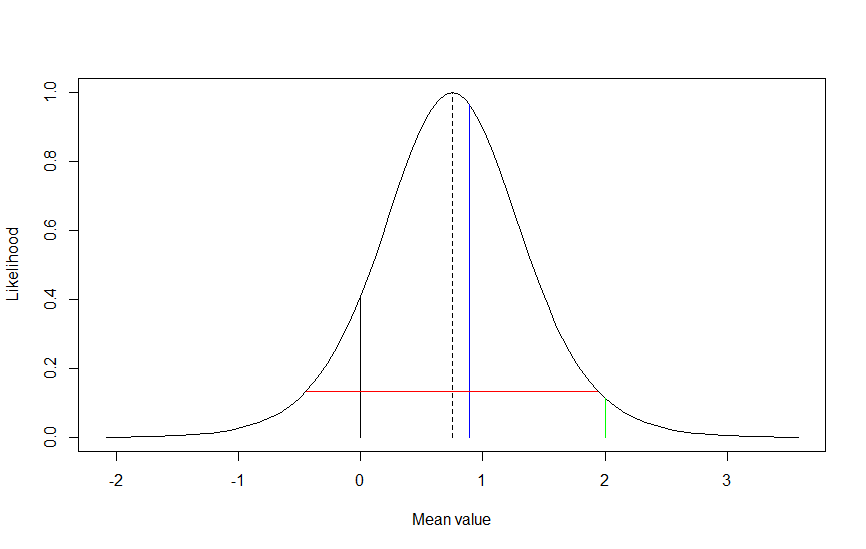
\includegraphics[width=12cm,
  keepaspectratio,]{figure1}
\caption{Graphical output from running the one-sample test function \texttt{L\_ttest}. The likelihood function for the mean value given the data, with the MLE (sample mean) represented by the vertical dashed line. The black line is the specified null value (here at 0), the blue line is for a specified alternative hypothesis (for an effect size of 0.5), and the green line represents a second alternative hypothesis (for 2 hours). The red horizontal line shows the \emph{S}-2 likelihood interval.}
\label{figure:figure1}
\end{figure}
The assigned object \texttt{a1} contains values of interest which can be assessed in the usual way with a1\$..., but entering \texttt{a1} on its own gives all the values:

\begin{tabular}{ll}  
\texttt{\$obs.mean} & the observed mean or difference in mean for related samples\\  
\texttt{\$df} & degrees of freedom\\  
\texttt{\$alt.H1} & mean value according to specified d\\ 
\texttt{\$alt.H2} & specified second hypothesis value\\
\texttt{\$S\_max} & maximum support for observed mean against the null\\
\texttt{\$S\_10} & support for d versus null\\
\texttt{\$S\_12} & support for d versus specified second hypothesis\\
\texttt{\$S\_20} & support for second hypothesis versus the null\\
\texttt{\$like.int} & likelihood interval\\
\texttt{\$L.int.spec} & specified likelihood interval in units of support\\
\texttt{\$null.value} & null value\\
\texttt{\$t.val} & t value for test against null\\
\texttt{\$p.val} &\emph{p} value for test against null\\
\texttt{\$d.obs} & observed effect size\\
\end{tabular}\\\\
For the related sample test a second vector of values of equal length to data1 (and paired) is entered for \texttt{data2}.  The independent samples test function is \texttt{L\_2S\_ttest}. The data is entered as the first argument followed by the vector of the same length coding groups. Similar arguments to the one sample/related sample test can be specified and similar output, but this time showing the difference in means.\\
The package includes one-way ANOVA (\texttt{L\_1way\_ANOVA}), one-way repeated measures ANOVA (\texttt{L\_1way\_RM\_ANOVA}) and two-way between-participants factorial ANOVA (\texttt{L\_2way\_Factorial\_ANOVA}). All these functions use contrasts, employing the model comparison approach espoused by Glover and Dixon \citep{Dixon:2003,GloverDixon:2004,Dixon:2013}. For the one-way analyses if the arguments for the contrasts are not specified then they default to testing a linear and a quadratic contrast. In the factorial ANOVA, no contrast comparisons are made if the contrasts are left unspecified. If the first contrast is specified then this is compared to the main effects, and if the second contrast is specified then this is compared to the first contrast. Such contrast comparisons are easy to do in this approach, and are difficult or impossible to do using frequentist \emph{p} values. The support values for the between-participants analyses are adjusted using Akaike's correction \citep{HurvichTsai:1989}. We will look at \texttt{L\_2way\_Factorial\_ANOVA}. The first line of output gives the S for comparing the full model of main effects and interaction with the null model. Using data from \citet{Cahusac:2020} p 91\\

\begin{example}
> time <- c(6.4, 4.6, 6.4, 5.6, 5.9, 6.1, 6.3, 4.5, 4.8, 6.6, 7, 9.3, 7.9, 9.4, 8.2,
          4.4, 4.2, 5, 6.9,4.5, 4, 4.3, 6.9, 5.5, 5.8, 4.4, 4.2, 5.1, 6.9, 4.5)
> Treatment = gl(3,5,30, labels=c("T1","T2","T3"))
> Health = gl(2,15,30, labels=c("Hemophiliac","Normal"))
> contrast1 <- c(-1, -1, 5, -1, -1, -1) # interaction Hemo T3 higher than others
> contrast2 <- c(-1, -1, -1, 1, 1, 1)    # main effect of health status (Hemo higher)
> m1=L_2way_Factorial_ANOVA(time, Treatment, Health, contrast1, contrast2, verb=TRUE)

Support for full model (including interaction) versus null = 7.036
 Support for full model versus main effects = 2.968
 Support for contrast 1 versus main effects = 7.587
 Support for contrast 1 versus contrast 2 = 8.462

First factor main effect F(2,24) = 5.039, p = 0.01488452, partial eta-squared = 0.296
 Second factor main effect F(1,24) = 15.992, p = 0.0005281828, partial eta-squared = 0.4
 Interaction F(2,24) = 6.219, p = 0.006664992, partial eta-squared = 0.341
 Contrast 1 F(1,24) = 36.048, p = 3.373928e-06
\end{example}
\begin{figure}[htbp]
\centering
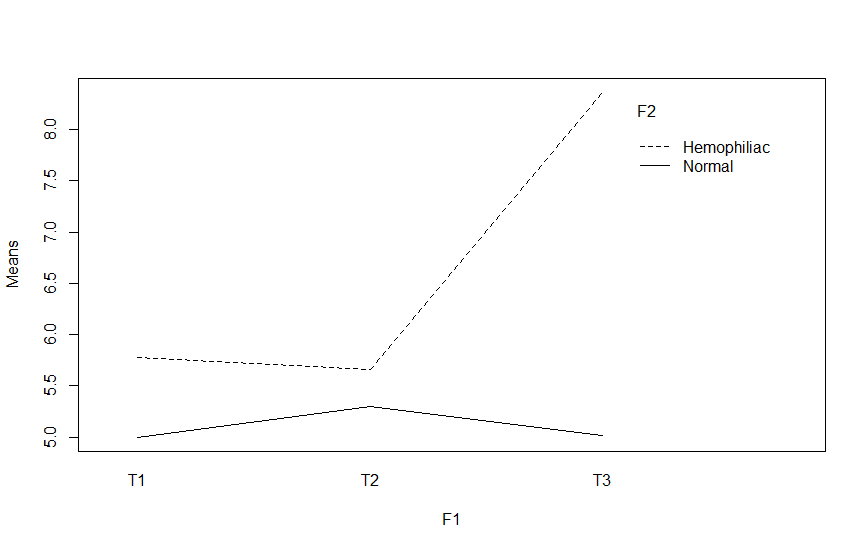
\includegraphics[width=12cm,
  keepaspectratio,]{figure2}
\caption{Graphical output from running the \texttt{L\_2way\_Factorial\_ANOVA} function. The interaction plot shows the means for the 2 groups of patients (dashed line is hemophiliac, solid line is normal). The horizontal axis represents the 3 different treatments. An interaction is apparent from the plot, where the 3rd treatment shows a clear difference between the hemophiliac and normal patients.}
\label{figure:figure2}
\end{figure}
As before, the assigned object \texttt{m1} contains values of interest which can be assessed in the usual way with \texttt{m1\$}..., but entering \texttt{m1} on its own gives all the values.\\
Bivariate normal correlation uses the \texttt{L\_corr function}, and is demonstrated by using data from the heptathlon \citep{Cahusac:2020} p 104\\
\begin{example}
> m200 <- c(22.6,23.7,23.1,23.6,23.6,23.6,25.5,23.9,24.5,23.9,24.9,24.8,24.7,
          25.0,24.6,24.9,25.0,25.6,24.8,25.5,25.7,24.9,26.6,25.2,26.2)
> m800 <- c(128.5,126.1,124.2,132.5,134.7,132.5,138.5,127.9,133.7,132.2,136.1,142.8,
          125.8,131.5,137.1,134.9,146.7,133.9,146.4,144.0,133.4,138.0,139.2,137.3,163.4)
> m2=L_corr(m200, m800, null=0, exp.r=0.5, L.int=3, alpha=.05, verb=TRUE)

Support for observed correlation 0.6198 (dashed line) versus null of 0 (black line) = 5.776
 Support for specified correlation of 0.5 (blue line) versus observed r = -0.338
 Support for specified correlation versus null = 5.438
 S-3 likelihood interval (red line) is from 0.19968 to 0.8474

 P value = 0.00095 
 N = 25
\end{example}
\begin{figure}[htbp]
\centering
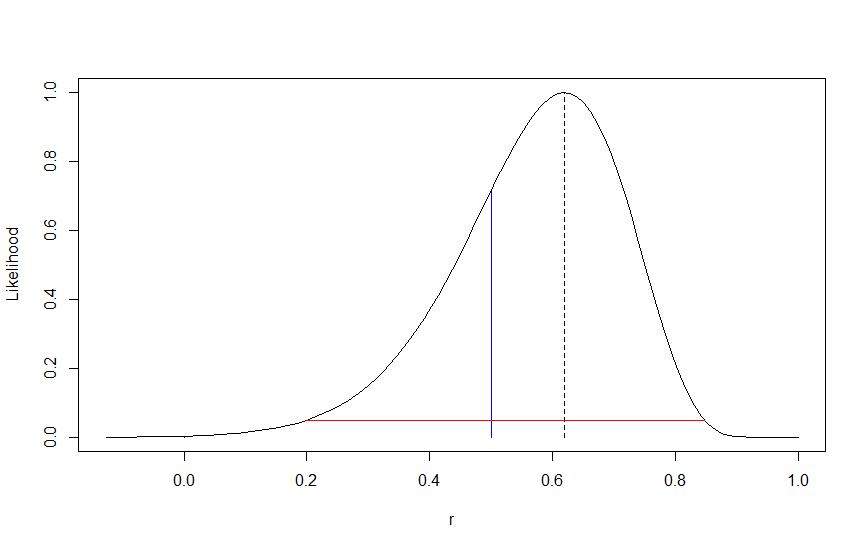
\includegraphics[width=12cm,
  keepaspectratio,]{figure3}
\caption{Graphical output from running the \texttt{L\_corr} function. This is the likelihood function for the correlation coefficient, given the data. As before, the vertical dashed line is the MLE (the sample \emph{r}), the blue line is a specified alternative value (0.5), and red horizontal line is the \emph{S}-3 likelihood interval. The null value at 0 is outside of this interval and the evidence against it is extremely strong. }
\label{figure:figure3}
\end{figure}
\pagebreak
The assigned object m2 contains values of interest which can be assessed in the usual way with m2\$..., but entering m2 on its own gives all the values.\\
The regression function \texttt{L\_regress} only accommodates one predictor, while the logistic regression function \texttt{L\_logistic\_regress} allows up to 6 predictors, which need to be dummy coded for nominal data with more than 2 levels.

\section{Categorical data}
There are 5 different tests included in the package (excluding logistic regression mentioned above). The simplest is the one-way categorical data analysis using the function \texttt{L\_1way\_cat}. Two categories represents the binomial (giving the likelihood function plot), while multiple categories represents the multinomial distribution. The two-way categorical analysis uses the \texttt{L\_2way\_cat} function. For these two functions an additional evidence-based statistic S for the variance is calculated. This uses the formula given by \citet{Cahusac:2020} p 158 and derived from \citet{Edwards:1992} p 187:\\
\begin{equation} \label{eqn}
S = \frac{df}{2} \left( log \frac{df}{\chi_{df}^{2}} \right) - \frac{1}{2}(df - \chi_{df}^{2}),
	\end{equation}
where \emph{df} is the degrees of freedom. This is most useful to test the variance in the model, specifically whether data are "too good to be true", i.e. the data fit a particular hypothesis closer than we would expect by chance \citep{Edwards:1986}. Using just 2 categories in the one-way analysis can be demonstrated:\\
\begin{example}
> obs <- c(18,5); exp.p <- c(0.7, 0.3)  # observed and expected values
> m3 <- L_1way_cat(obs, exp.p, verb = TRUE)

Binomial support for difference of MLE 0.7826087 (dashed line) 
 from 0.7 (blue line) with 1 df = 0.398
 Support for variance differing more than expected = 0.019

 S-2 likelihood interval (red line) from 0.5853 to 0.91794

Chi-square(1) = 0.747,  p = 0.3872968
 Likelihood ratio test G(1) = 0.795, p = 0.37258, N = 23
 Likelihood-based 95% confidence interval from 0.58958 to 0.91597
\end{example}

\begin{figure}[htbp]
\centering
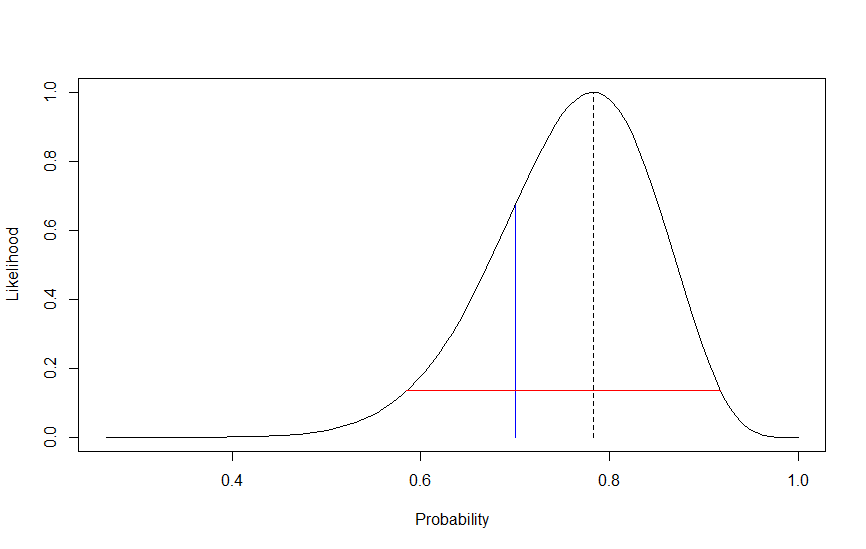
\includegraphics[width=12cm,
  keepaspectratio,]{figure4}
\caption{Graphical output from running the \texttt{L\_1way\_cat} function. This shows the likelihood function for the proportion, given the data. The vertical dashed line is the MLE, the blue line is the alternative hypothesis value (0.7), and the red horizontal line is the \emph{S}-2 likelihood interval.}
\label{figure:figure4}
\end{figure}
As previously, the assigned object \texttt{m3} contains values of interest which can be assessed in the usual way with \texttt{m3\$}..., but entering \texttt{m3} on its own gives all the values.\\
Some of the functions provide likelihood-based \% confidence interval \citep{Aitkin:1989}.\\
Finally, there are functions to calculate the odds ratio \texttt{L\_OR}, relative risk \texttt{L\_RR} and binomial efficacy \texttt{L\_efficacy}.

\section{Sample size calculations}
The main challenge faced by the evidential researcher is of obtaining sufficiently strong evidence for or against one of two specified hypotheses. Like the probability of a Type II error, this probability is large with a small sample size and decreases as sample size increases. The function \texttt{L\_t\_test\_sample\_size} can be used to calculate the pre-study sample size for all the \emph{t} tests \citep{Cahusac:2022}. The combined misleading and weak probability \citep{Royall:1997,Royall:2000,Royall:2004} is entered, with a default of 0.05, together with the strength of evidence desired (default = 3). For a paired samples test, where we wish to calculate sample size with a combined .2 probability of obtaining misleading or weak evidence, strength of evidence \emph{S} = 2 and effect size 0.5, we would obtain a value of 38 by using the following:\\
\begin{example}
> L_t_test_sample_size(MW = 0.2, sd = 1, d = 0.5, S = 2, paired = TRUE)

For 1 sample, or related samples, t test with M1 + W1 probability of 0.2
 Strength of evidence required is 2, and effect size of 0.5
 Required sample size = 38
 \end{example}
 
The somewhat comparable calculation for Type II error of 0.2, two-sided alpha = 0.05 and same effect size of 0.5 produces a sample size of 34 (using stats::power.t.test(power = .80, delta = 0.5, sig.level=0.05, type="paired")). 
 
\section{Conclusions}
The functions described for the likelihoodR package may be useful for those researchers and statisticians who wish to use the evidential approach for their data analysis \citep{Cahusaca:2020}. In addition to the advantages mentioned earlier in the introduction there are other desirable features. First, categorical data analyses are not restricted by normality assumptions, and support values for independent components of cross-tabulated data sum precisely and algebraically (unlike such calculations in chi-square analyses). Second, in categorical and measurement analyses it is possible to show that the data fit the null (or other) hypothesis too well (e.g. for detection of data fraud). Third, analyses are versatile with unlimited complexity for model comparisons within a dataset, for example in ANOVA \citep{GloverDixon:2004}.\\
As far as the author is aware, no other packages are available in R or other platforms. Currently users calculate likelihood ratios manually. This package addresses this shortcoming and hopefully will encourage more users to express their results in terms of log likelihood ratios.\\ 
One of the products of the likelihoodR package is that a module has been developed for jamovi \citep{jamovi}, named \textbf{jeva}, which includes many of these functions. Hopefully this will encourage further interest in the likelihood approach and facilitate teaching and research. The equivalent jamovi analysis is given earlier for the \texttt{L\_ttest} produces output given in Figure 5. The output produced by jamovi is identical to that produced earlier by the package, although simpler in that it lacks the option of comparing an effect size (d, illustrated by the blue line in package output). The null versus observed (1st line of Support output) is -0.892, while in the package it is 0.892, the positive value being due to comparing observed versus the null. Other outputs match apart from decimal rounding, which can be selected in jamovi. The \emph{t}, degrees of freedom (df) and \emph{p} are the same for the null versus observed, although the jamovi output includes another line giving these statistics for the alternative hypothesis versus the observed. The jamovi output includes group descriptive statistics (although these are available from the assigned object in the package, e.g. \texttt{\$obs.mean}. The jamovi output also includes the option of a descriptives plot (not shown) which displays the mean with specified likelihood interval.\\
The likelihoodR package described in this article provides a large number of functions, currently many more than envisaged for the jamovi module. As such, it will provide a major reference package for users interested in the likelihood approach.\\

\begin{figure}[htbp]
\centering
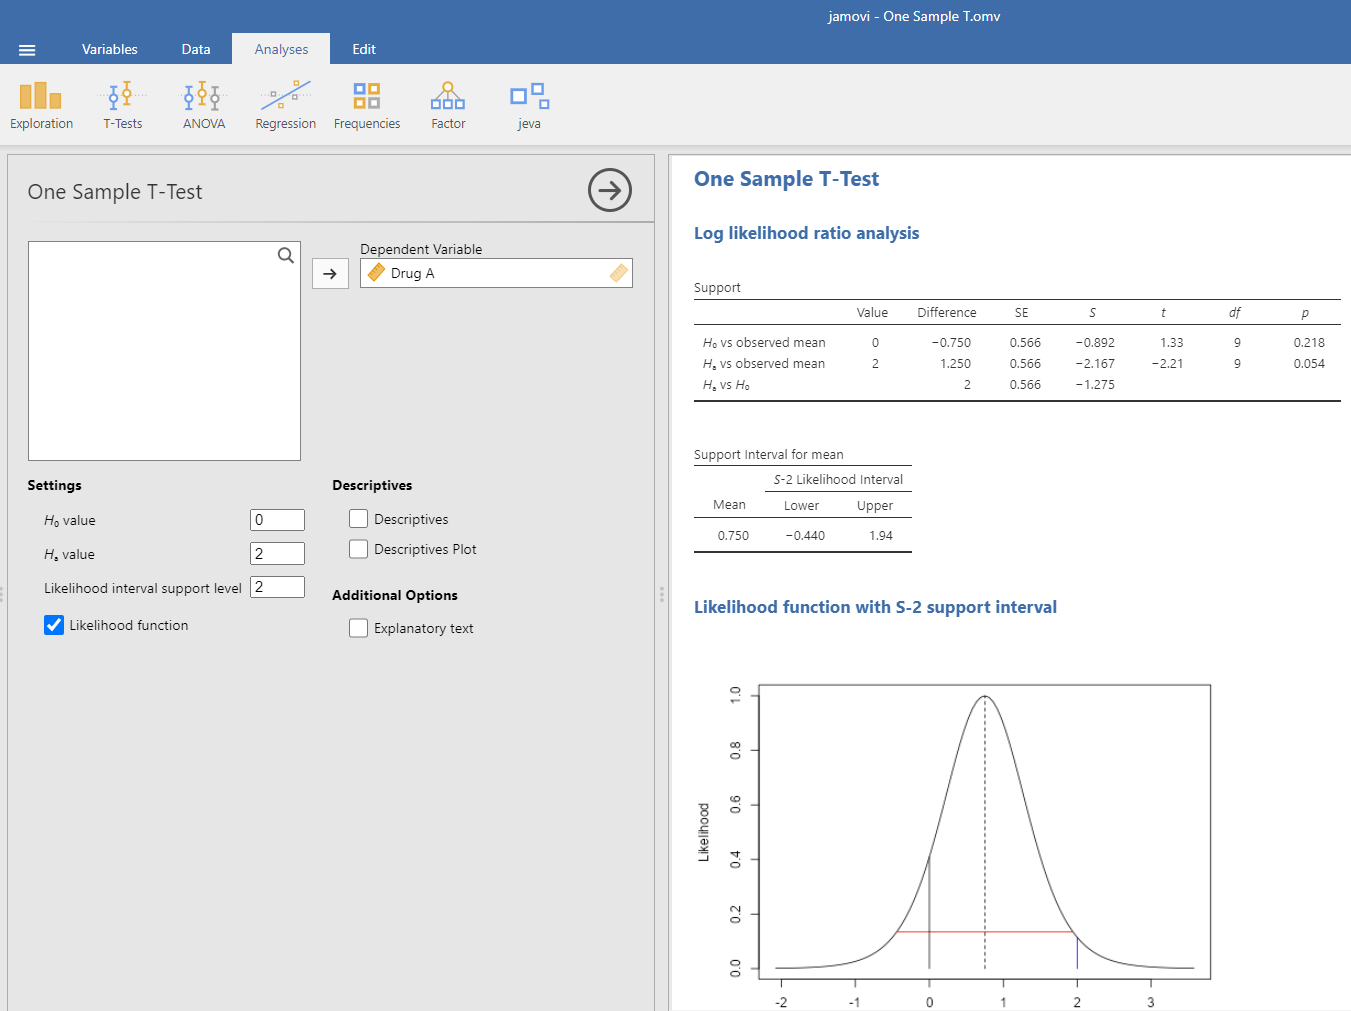
\includegraphics[width=15cm,
  keepaspectratio,]{figure5}
\caption{Graphical output from running the one-sample \emph{t} test in the jamovi module \textbf{jeva} (created from the \texttt{L\_ttest} function). The screenshot should be compared directly with Figure 1. On the left side is the dialog box where a variable can be selected (Drug A), and various settings chosen, including the null and alternative hypothesis values, and to display the likelihood function. An additional option gives an explanation about the obtained support values and likelihood interval, and their interpretation. On the right side is a summary of the analysis, at the top showing the \emph{S} values for hypothesis comparisons (see text for the interpretation of the tabulated values). Below this is shown the support interval, and finally below that the likelihood function. The line colours for the likelihood function are the same as those given in Figure 1, although there is no option for a specified effect size (no green line). }
\label{figure:figure5}
\end{figure}
\pagebreak
\bibliography{Cahusac}
\address{Peter Cahusac\\
  College of Medicine, Alfaisal University, Riyadh\\
  Department of Pharmacology \& Biostatistics\\
  And Department of Comparative Medicine\\
  King Faisal Specialist Hospital \& Research Centre, Riyadh\\
  Kingdom of Saudi Arabia\\
  ORCiD 0000-0003-4976-2834\\
  \email{pcahusac@alfaisal.edu}}
